%!TEX root = ../Thesis.tex
\section{Frontend-Implementierung}
Das Frontend der Anwendung ist in drei wesentliche logische Abschnitte eingeteilt. Der erste Teil ist die Authorisierung, welcher für Abfragen von 
Credentials und der Speicherung dieser zuständig ist. Der zweite Teil verwendet die Credentials dann um auf die API zuzugreifen, und benötigte 
Daten zu extrahieren. Diese Daten werden dann im dritten Teil, dem User Interface, verwendet. 
\subsection{Authorisierung}
Im Sinne der Erweiterbarkeit und Wartbarkeit wurde folgende Ordnerstruktur gewählt:\break
\begin{center}
    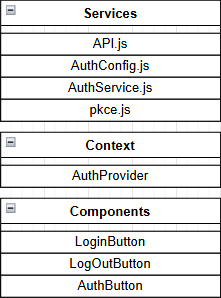
\includegraphics[width=\linewidth]{./img/fileStructure.png}
\end{center}


Der Login-Prozess wird in drei semantische Kategorien aufgeteilt. An erster Stelle stehen die Komponenten,
die dem User die Interaktion mit der Authorisierungs-Logik ermöglichen. 
\subsubsection{Components}
Obwohl theoretisch auch eine einzelne Komponente für den Login-Prozess ausreichen würde, wurde der Login/Logout-Button
im Sinne der Übersichtlichkeit getrittelt. Der Login- sowie Logout-Button sind sind in der Logik bis auf die ausgeführte Methode identisch:
\begin{figure}[H]
    \begin{lstlisting}[caption=JS-Code for the LogIn-Button, label=list:loginbutton]
        // components/LoginButton.js
        import React from 'react';
        import { useAuth } from '../context/AuthContext';
        import { Button } from '@element/react-components';

        export default function LoginButton() {
            const { login } = useAuth();

            return <Button onClick={login} label="Log In"/>
        }
    \end{lstlisting}
    %\footnoterule{}
    %\footnotesize{Casts have been omitted for the sake of readability}
\end{figure}
Der Login-Button, welcher aus der Unternehmens-internen React-Bibliothek entnommen wird, ruft bei Interaktion die \texttt{login()}-Methode 
aus dem Authentifizierungs-Kontext auf, welcher im nächsten Abschnitt beschrieben wird.\break
Der gleiche Prozess findet beim Logout-Button statt, nur dass hier die \texttt{logout()}-Methode aufgerufen wird.
\begin{figure}[H]
    \begin{lstlisting}[caption=JS-Code for the LogOut-Button, label=list:logoutbutton]
        // components/LogoutButton.js
        import React from 'react';
        import { useAuth } from '../context/AuthContext';
        import { Button } from '@element/react-components';

        export default function LogoutButton() {
            const { logout } = useAuth();

            return <Button onClick={logout} label="Log Out"/>
        }
    \end{lstlisting}
    %\footnoterule{}
    %\footnotesize{Casts have been omitted for the sake of readability}
\end{figure}
Diese beiden Komponenten werden dann im AuthButton kombiniert, wobei der Auth-Status entscheidet, 
welcher Button angezeigt wird:
\begin{figure}[H]
    \begin{lstlisting}[caption=JS-Code for the AuthButton, label=list:authbutton]
        // components/AuthButton.js
        import React from 'react';
        import { useAuth } from '../context/AuthContext';
        import LoginButton from './LoginButton';
        import LogoutButton from './LogoutButton';

        export default function AuthButton() {
            const { isAuthenticated } = useAuth();

            return isAuthenticated ? <LogoutButton /> : <LoginButton />;
        }
    \end{lstlisting}
    %\footnoterule{}
    %\footnotesize{Casts have been omitted for the sake of readability}
\end{figure}
Für die Entscheidung, welcher Button angezeigt wird, wird zuerst über die \texttt{useAuth()}-Hook\footnote{In JavaScript, speziell in React, ist eine Hook eine Funktion, mit der ein Zugriff auf React-Features wie State oder Lifecycle-Methoden in Funktionskomponenten möglich gemacht wird}
der Authentifizierungs-Kontext abgerufen. Der daraus resultierende Boolean-Wert \texttt{isAuthenticated} gibt an, ob der User eingeloggt ist oder nicht.
Mit diesem Boolean-Wert wird dann entschieden, ob der Login- oder Logout-Button angezeigt wird. Das geschieht in diesem Fall mithilfe eines ternären Operators,
der den Wert von \texttt{isAuthenticated} überprüft und abhängig vom Wert den entsprechenden Button zurückgibt.\footnote{\url{https://developer.mozilla.org/en-US/docs/Web/JavaScript/Reference/Operators/Conditional_operator}}
\subsubsection{Context}
Der Authentifizierungs-Kontext ist ein zentraler Bestandteil der Authorisierungs-Logik. Er stellt die Methoden \texttt{login()} und \texttt{logout()} 
zur Verfügung, ist aber zusätzlich auch für die Verarbeitung des Callbacks von Cognito zuständig.
Zuerst werden für den Kontexst die benötigten Hooks importiert und ein Context-Objekt erstellt:
\begin{figure}[H]
    \begin{lstlisting}[caption=Import und Kontext, label=list:authcontextimports]
        import React, { createContext, useState, 
        useEffect, useContext } from 'react';
        import { useNavigate, useLocation } from 'react-router-dom';
        import {buildAuthUrl, generateChallenge, generateVerifier, 
        exchangeCodeForTokens} from '../service/authService';
        import authConfig from '../services/authConfig';
        import {generateVerifier, generateChallenge} from '../service/pkce';

        const AuthContext = createContext();
    \end{lstlisting}
\end{figure}
Daraufhin werden für den Kontext relevante Variablen definiert, die den User, den Authentifizierungsstatus und die Tokens enthalten:
\begin{figure}[H]
    \begin{lstlisting}[caption=Variablen für den Authentifizierungs-Kontext, label=list:authcontextvariables]
        const [user, setUser] = useState(null);
        const [isAuthenticated, setIsAuthenticated] = useState(false);
        const [tokens, setTokens] = useState(null);
        const navigate = useNavigate();
        const location = useLocation();
    \end{lstlisting}
\end{figure}
Die \texttt{login()}-Methode generiert einen zufälligen State und einen PKCE-Verifier, speichert diese im Session Storage und 
leitet den User zur Authentifizierungs-URL weiter:
\begin{figure}[H]
    \begin{lstlisting}[caption=Login-Methode, label=list:authcontextlogin]
        async function login() {
            const state = crypto.randomUUID();
            const verifier = generateVerifier();
            const challenge = await generateChallenge(verifier);

            sessionStorage.setItem('oauth_state', state);
            sessionStorage.setItem('pkce_verifier', verifier);
            
            const url = buildAuthUrl({state, code_challenge: challenge});

            window.location.href = url;
        }
\end{lstlisting}
\end{figure}
Die \texttt{logout()}-Methode löscht den Session Storage und leitet den User zur Logout-URL weiter:
\begin{figure}[H]
    \begin{lstlisting}[caption=Logout-Methode, label=list:authcontextlogout]
        function logout() {
            sessionStorage.clear();
            const {logoutEndpoint, clientId, logoutUri} =authConfig;
            window.location.href = `${logoutEndpoint}?client_id=${clientId}&logout_uri=${encodeURIComponent(logoutUri)}`; 
        }
    \end{lstlisting}
\end{figure}
Die \texttt{handleCallback()}-Methode wird aufgerufen, wenn der User nach der Authentifizierung zurück zur Anwendung geleitet wird.
Das wird durch die \texttt{useEffect()}-Hook realisiert, die prüft, ob der User auf der Callback-Route ist und ob ein Code in der URL vorhanden ist.
\begin{figure}[H]
    \begin{lstlisting}[caption=Callback-Handling, label=list:authcontextcallback]
        useEffect(() => {
            if (location.pathname === '/callback' && location.search.includes('code=')) {
                handleCallback();
            }
        }, [location, handleCallback]);
\end{lstlisting}
\end{figure}
Die \texttt{handleCallback()}-Methode extrahiert den Code und den State aus der URL, vergleicht den State mit dem im Session Storage gespeicherten Wert und tauscht den Code gegen Tokens aus.
Falls der Austausch erfolgreich ist, werden die Tokens im Zustand gespeichert und der User wird zur Dashboard-Seite weitergeleitet:
\begin{figure}[H]
    \begin{lstlisting}[caption=Callback-Handling, label=list:authcontextcallback2]
        async function handleCallback() {
            const params = new URLSearchParams(location.search);
            const code = params.get('code');
            const state = params.get('state');
            const saved = sessionStorage.getItem('oauth_state');

            if(!code || !state || state !== saved) {
                return navigate('/', {replace: true});
            }

            try{
                const verifier = sessionStorage.getItem('pkce_verifier');
                const tokenSet = await exchangeCodeForTokens(code, verifier);
                setTokens(tokenSet);

                const [, payload] = tokenSet.id_token.split('.');
                const userInfo = JSON.parse(atob(payload));
                setIsAuthenticated(true);

                sessionStorage.removeItem('pkce_verifier');
                sessionStorage.removeItem('oauth_state');

                navigate('/dashboard', {replace: true});
            } catch (err) {
                console.error('Error during authentication:', err);
                navigate('/', {replace: true});
            }
        }
    \end{lstlisting}
\end{figure}
Die \texttt{AuthProvider}-Komponente stellt den Authentifizierungs-Kontext für die gesamte Anwendung bereit:
\begin{figure}[H]
    \begin{lstlisting}[caption=AuthProvider-Komponente, label=list:authcontextprovider]
        return (
            <AuthContext.Provider 
            value={{ user, isAuthenticated, tokens, login, logout }}>
                {children}
            </AuthContext.Provider>
        );
    }
    export function useAuth() {
        return useContext(AuthContext);
    }
    \end{lstlisting}
\end{figure}
Die \texttt{useAuth()}-Hook ermöglicht den Zugriff auf den Authentifizierungs-Kontext in anderen Komponenten der Anwendung.
\subsubsection{Service}    
Der Service-Ordner enthält unterstützende Funktion für die Authorisierung, wie die Generierung des PKCE-Verifiers 
und -Challenges, den Austausch des Codes gegen Tokens und die Estellung der Authentifizierungs-URL.
Zuerst muss dafür die Konfiguration definiert werden, mit der gearbeitet wird.
\subsubsection{AuthConfig}
Die \texttt{authConfig.js}-Datei enthält die Konfiguration für die Authentifizierung, einschließlich der Endpunkte, Client-ID und Redirect-URI. 
Zusätzlich wird auch die Basis-URL der API definiert, um später API-Anfragen zu ermöglichen:
\begin{figure}[H]
    \begin{lstlisting}[caption=AuthConfig, label=list:authconfig]
        const domain = process.env.REACT_APP_COGNITO_DOMAIN;
        const clientId = process.env.REACT_APP_COGNITO_CLIENT_ID; 
        const redirectUri = process.env.REACT_APP_COGNITO_REDIRECT_URI;
        const logoutUri = process.env.REACT_APP_COGNITO_LOGOUT_URI;
        const apiBaseUrl = process.env.REACT_APP_API_BASE_URL;
        export const authConfig = {
            domain,
            clientId,
            redirectUri,
            logoutUri,
            apiBaseUrl: apiBaseUrl,
            authEndpoint: `https://${domain}/oauth2/authorize`,
            tokenEndpoint: `https://${domain}/oauth2/token`,
            logoutEndpoint: `https://${domain}/logout`,
            responseType: 'code',
            scope: 'openid profile email',
        };
    \end{lstlisting}
\end{figure}
Mit dieser Konfiguration wird nun gearbeitet, um alle weiteren benötigten Daten zu generieren.
\subsubsection{AuthService}
Der AuthService enthält drei Methoden, die für die Authorisierung benötigt werden:
\begin{itemize}
    \item \texttt{buildAuthUrl()}: Diese Methode generiert die Authentifizierungs-URL, die den User zur Cognito-Anmeldeseite weiterleitet.
    \item \texttt{exchangeCodeForTokens()}: Diese Methode tauscht den erhaltenen Code gegen Tokens aus, die für die Authentifizierung und Autorisierung verwendet werden.
    \item \texttt{refreshTokens()}: Diese Methode aktualisiert die Tokens, wenn sie abgelaufen sind.
\end{itemize}
Die \texttt{buildAuthUrl()}-Methode erstellt die Authentifizierungs-URL, indem sie die Konfiguration und die PKCE-Challenge verwendet:
\begin{figure}[H]
    \begin{lstlisting}[caption=Build-Auth Methode, label=list:buildAuth]
        export function buildAuthUrl({state, code_challenge}) {
            const {
                authorizeEndpoint,
                clientId,
                redirectUri,
                responseType,
                scope
            } = authConfig;
            const params = new URLSearchParams({
                client_id: clientId,
                redirect_uri: redirectUri,
                response_type: responseType,
                scope,
                state,
                code_challenge_method: 'S256',
                code_challenge
            });
            return '${authorizeEndpoint}?{params}';
        }
    \end{lstlisting}
\end{figure}
Die \texttt{exchangeCodeForTokens()}-Methode tauscht bei Rückruf von der Cognito-Authentifizierung den mitgegebenen Code für ein gültiges
Auth-Token. Dieses kann dann verwendet werden, um API-Abfragen durchzuführen:
\begin{figure}[H]
    \begin{lstlisting}[caption=ExchangeCodeForToken Methode, label=list:exchangecodefortoken]
        export async function exchangeCodeForToken(code, code_verifier){
            const {tokenEndpoint, clientId, redirectUri} = authConfig;

            const params = new URLSearchParams({
                grant_type: 'authorization_code',
                client_id: clientId,
                code,
                redirect_uri: redirectUri,
                code_verifier
            });

            const resp = await fetch(tokenEndpoint, {
                method: 'POST',
                headers: {'Content-Type': 'application/x-www-form-urlencoded' },
                body: params.toString()
            });

            const text = await resp.text();

            if(!resp.ok) throw new Error('Token Exchange failed: $(text)')
            return JSON.parse(text);
        }
    \end{lstlisting}
\end{figure}
Dafür werden zuerst die nötigen Konfigurations-Daten geladen und die Parameter für die URL-Suche definiert. Mit diesen Daten wird dann 
eine Anfrage an den TokenEndpoint gesendet und die Antwort als das Token zurückgegeben, sollten keine Fehler auftreten.
\subsubsection{PKCE}
PKCE(Proof Key for Code Exchange) ist eine Erweiterung des OAuth 2.0-Protokolls, welches zusätzliche Sicherheit für Clients verspricht,
die nicht in der Lage sind, ihre Client-Geheimnisse sicher zu speichern.
Innerhalb dieser Anwendung wird PKCE verwendet, um den Authentifizierungsprozess sicherer zu gestalten. Dies geschieht über zwei Methoden,
\texttt{generateVerifier()} und \texttt{generateChallenge()}, die jeweils den Verifier und die Challenge generieren. \break

Die \texttt{generateVerifier()}-Methode generiert einen zufälligen Verifier, der als Basis für die Challenge dient. Das geschieht, indem 
ein Array von 32 zufälligen Bytes generiert wird, welches dann in einen hexadezimalen String umgewandelt wird:
\begin{figure}[H]
    \begin{lstlisting}[caption=PKCE-Verifier-Generierung, label=list:pkceverifier]
        export function generateVerifier() {
            const array = new Uint8Array(32);	
            crypto.getRandomValues(array);
            return Array.from(array, b => ('0'+ b.toString(16)).slice(-2)).join('');
        }
    \end{lstlisting}
\end{figure}
Die \texttt{generateChallenge()}-Methode nimmt den Verifier als Eingabe und generiert die Challenge, indem der Verifier in einen SHA-256-Hash umgewandelt wird.
Das Ergebnis wird dann in einen Base64-URL-kodierten String umgewandelt:
\begin{figure}[H]
    \begin{lstlisting}[caption=PKCE-Challenge-Generierung, label=list:pkcechallenge]
        export async function generateChallenge(verifier) {
            const encoder = new TextEncoder();
            const data = encoder.encode(verifier);
            const hash = await crypto.subtle.digest('SHA-256', data);
            return btoa(String.fromCharCode(...new Uint8Array(hash)))
                .replace(/\+/g, '-').replace(/\//g, '_').replace(/=+$/, '');
        }
    \end{lstlisting}
\end{figure}
\subsubsection{API}
Der API-Service ist die Hook \texttt{useApi()}, welche für die Kommunikation mit der Backend-API zuständig ist. 
Sie Kapselt die Methode \texttt{callAPI()} ab, welche den Zugriff auf die Konfigurierte API ermöglicht:
\begin{figure}[H]
    \begin{lstlisting}[caption=PKCE-Challenge-Generierung, label=list:pkcechallenge]
        async function callApi(path, options = {}){
            const url = '${authConfig.apiBaseUrl}${path}';
            const resp = await fetch(url, {
                ...options,
                headers: {
                    'Content-Type': 'application/json',
                    Authorization: 'Bearer ${tokens.access_token}',
                    ...options, headers
                }
            });
            if (!resp.ok) throw 
            new Error('API error ${resp.status}: ${await resp.text()}');
            return resp.json();
        }
    \end{lstlisting}
\end{figure}
Die Daten, die aus der \texttt{callApi()}-Methode zurückgegeben werden, können dann in den Komponenten verwendet werden, um die Daten anzuzeigen oder zu verarbeiten.
\subsection{User Interface}
Das User Interface der Anwendung ist in mehrere Komponenten 
 unterteilt, die jeweils für verschiedene Teile der Anwendung zuständig sind:\break
\begin{center}
    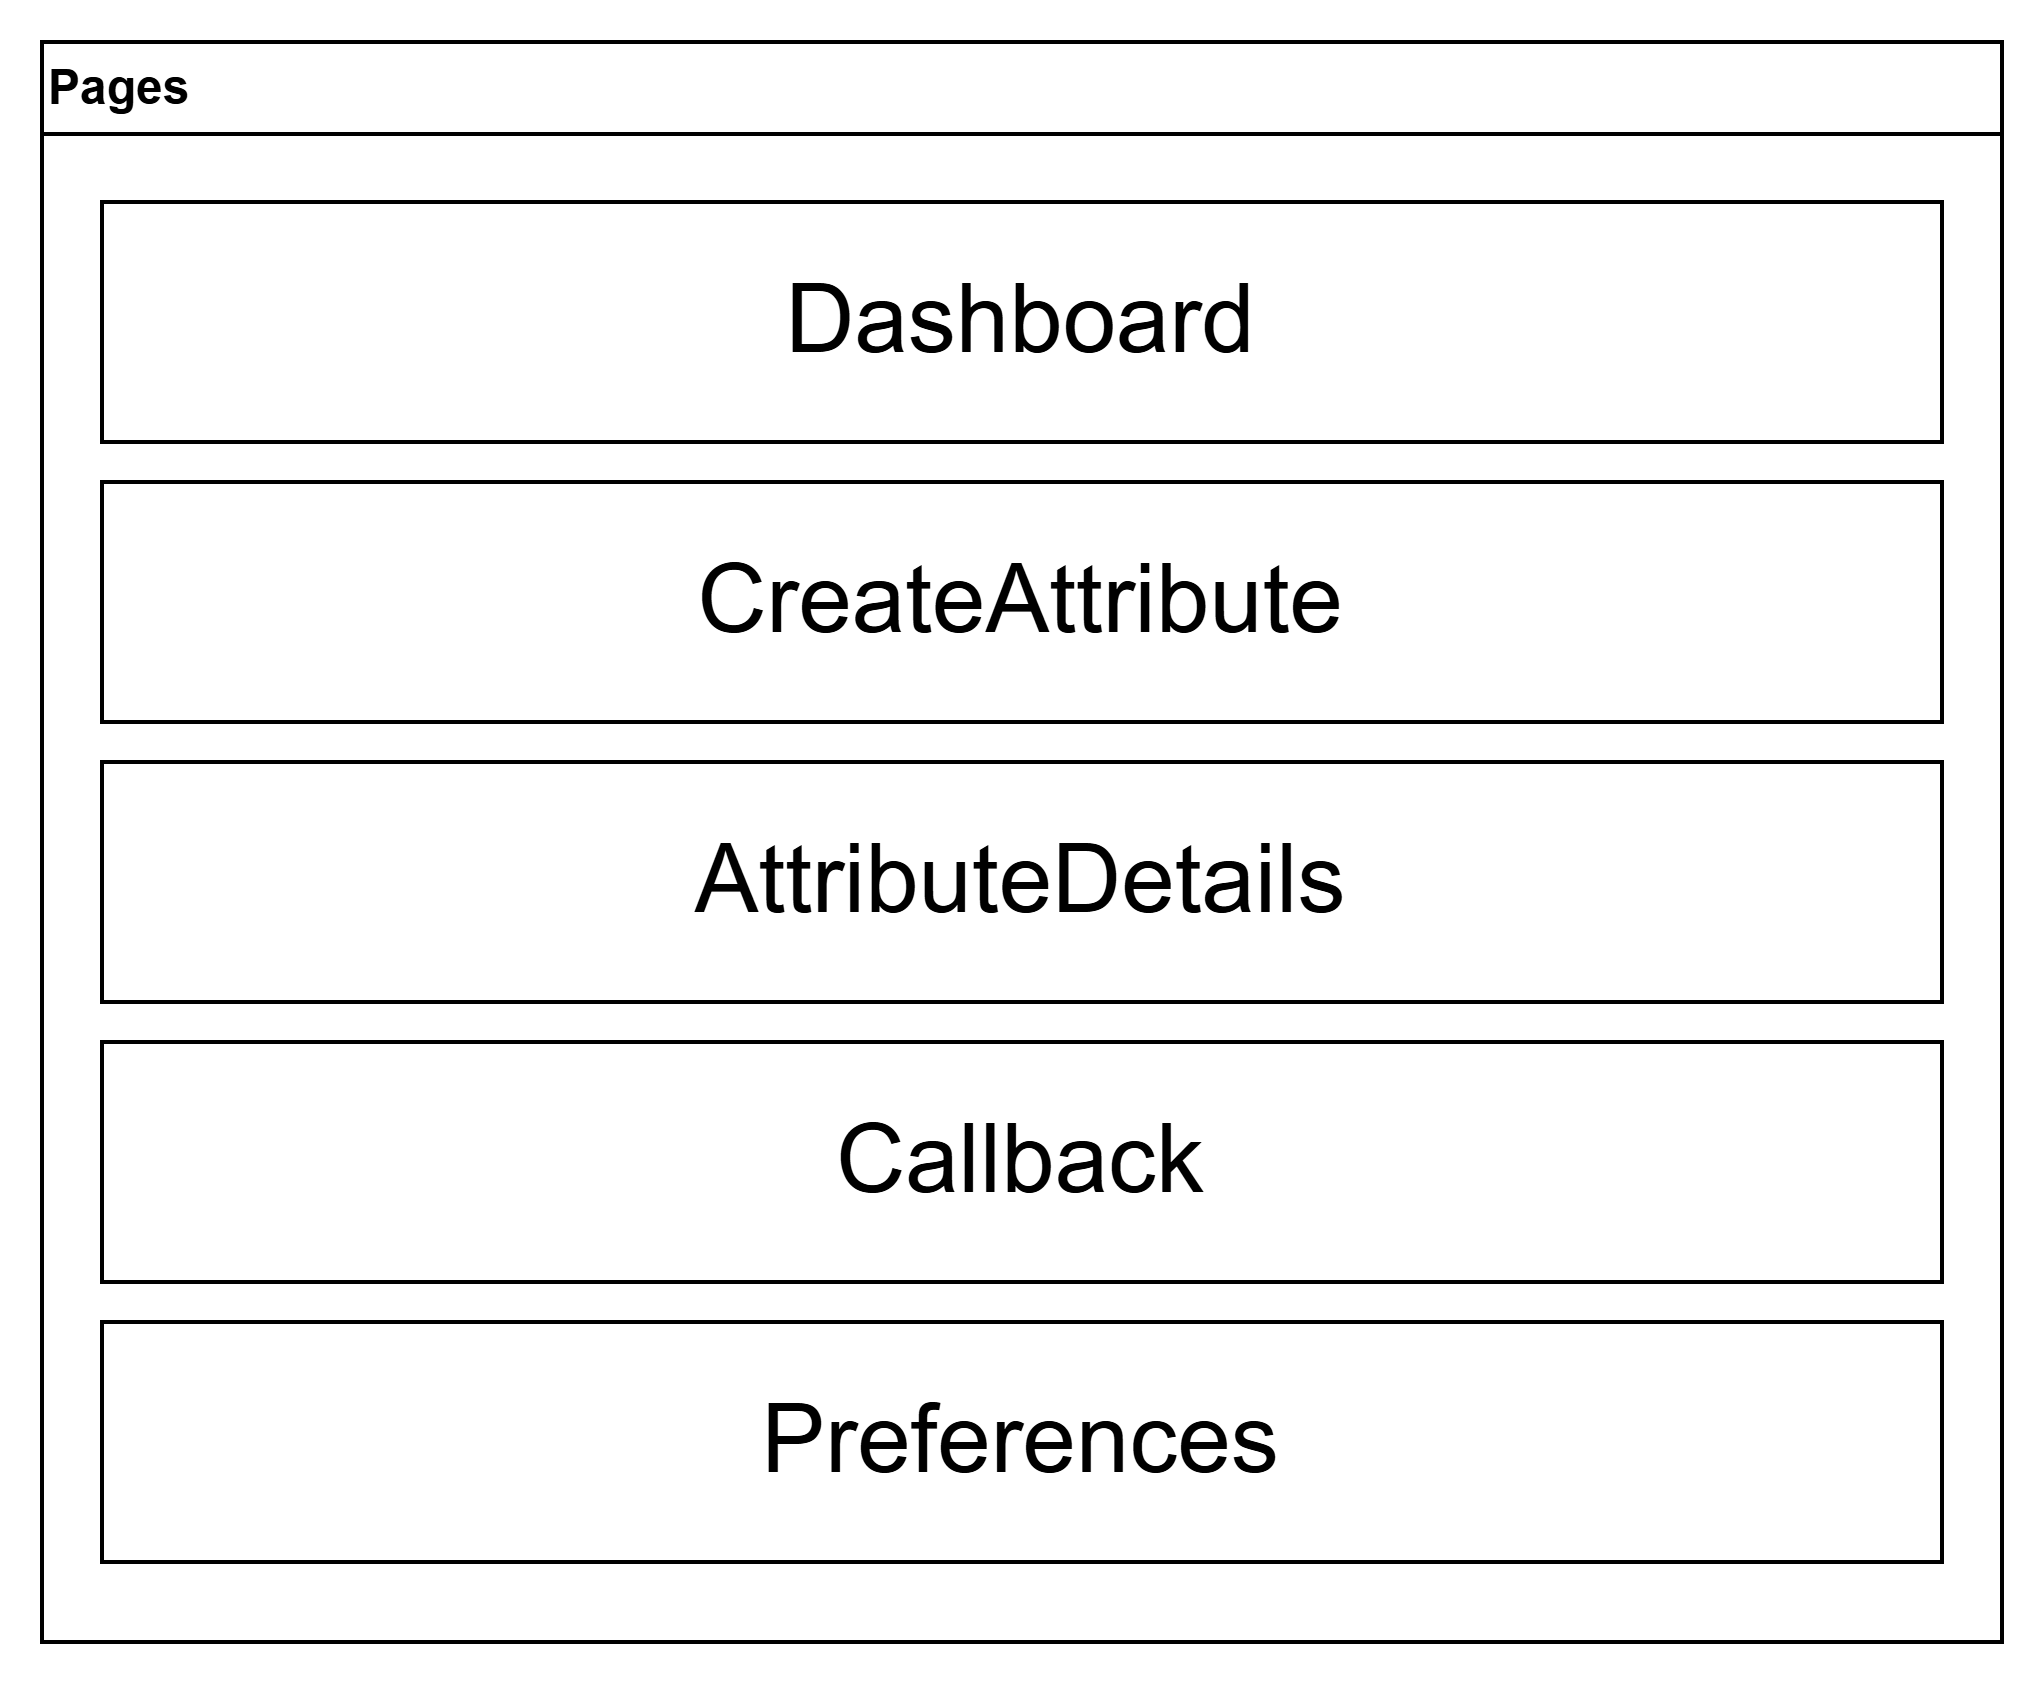
\includegraphics[width=\linewidth]{./img/dashboardFileStructure.png}
\end{center}
Den Kern der Anwendung bildet die \texttt{Dashboard}-Komponente, welche die Hauptansicht der Anwendung beinhaltet. Von hier aus werden die verscheidenen
Unterseiten aufgerufen (mit Ausnahme der Callback-Seite, die nur für die Authorisierung zuständig ist).
\subsection{Dashboard}
Das Dashboard teilt sich in drei Sektionen auf, mit denen der User seine Attribut-Wahl schrittweise konkretisieren kann. Die erste Sektion ist die Projekt-Auswahl,
welche in Form einer Navigationsleiste am oberen Rand der Seite dargestellt wird. Hier ist es wichtig, zwischen einem Projekt im Rahmen dieser Anwendung, und einem 
Projekt, wie es in der Newport\_Projects-Tabelle abgebildet ist, zu unterscheiden. Ein Projekt im Rahmen dieser Anwendung beinhaltet Daten aus allen Datenbanken des 
CSW, stellt also übergeordnet alle Komponenten einer Wirkstoff-Enwticklung dar. Ein Projekt in der Newport\_Projects-Tabelle hingegen beschränkt sich auf die Attribute
des Newport-Eintrags, der für den Wirkstoff angelegt wurde. Die folgende Abbildung stellt diese Unterscheidung dar:
\begin{center}
    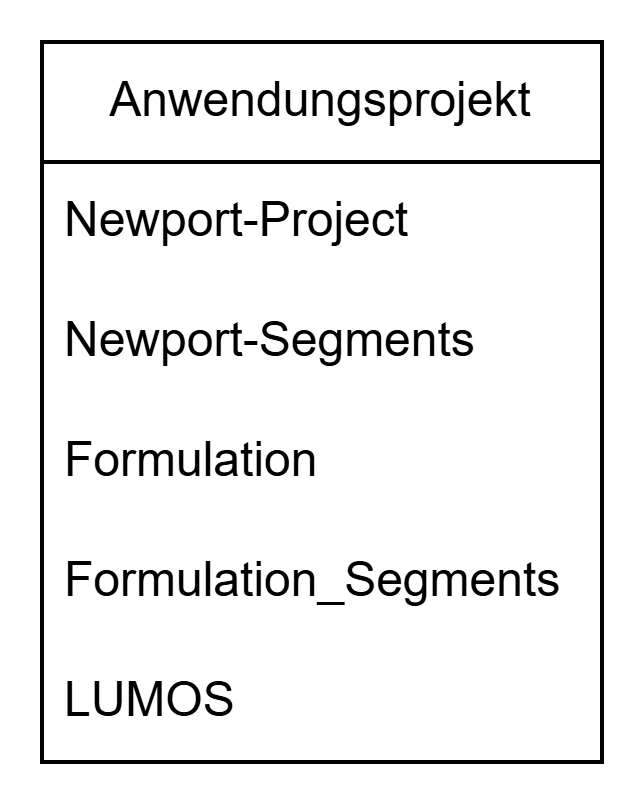
\includegraphics[width=\linewidth]{./img/projektGrafik.png}
\end{center}
Die zweite Sektion ist die Tabellen-Auswahl. Der User hat hier die Möglichkeit, zu entscheiden, welche der Tabellen des Anwendungsprojekts er um Attribute erweitern möchte.
Die dritte Sektion stellt die Attribute dar, die der Tabelle und dem Anwendungsprojekt zugeordnet sind. Hier kann der User Attribute auswählen, um diese zu bearbeiten, 
betrachten oder exportieren. Zusätzlich kann der User hier auch neue Attribute anlegen, die dann in dieser Ansicht angezeigt werden. Um ein neues Attribut anzulegen,
wird der Nutzer auf eine neue Seite weitergeleitet, auf der alle Daten für das neue Attribut eingegeben werden können.
\subsection{Attribut-Kreation}
Die Attribut-Kreation ist in mehrere Schritte unterteilt, die der User durchlaufen muss, um ein neues Attribut zu erstellen.
Auf der ersten Seite muss der User grundlegende Informationen zum Attribut angeben, worauf dann die weiteren Schritte angepasst werden.
Unter anderem muss der User hier den Name, die Beschreibung und den Typ des Attributs angeben. Dazu kommt auch die Angabe, ob das Attribut aus einem oder mehreren 
Werten bestehen soll. Diese Angabe ist wichtig, da sie die weiteren Schritte beeinflusst.
\begin{figure}[H]
    \begin{lstlisting}[caption=Attribut-Kreation, label=list:attributeCreation]
        <div>
            <label>Name:</label>
            <input type="text" value={name} 
            onChange={(e) => setName(e.target.value)} />
            <label>Beschreibung:</label>
            <input type="text" value={description} 
            onChange={(e) => setDescription(e.target.value)} />
            <label>Typ:</label>
            <select value={type} onChange={(e) => setType(e.target.value)}>
                <option value="string">String</option>
                <option value="number">Number</option>
                <option value="boolean">Boolean</option>
                <option value="date">Date</option>
            </select>
        </div>
    \end{lstlisting}
\end{figure}
Im zweiten Schritt muss der User dann den Wert populieren. Ob hier ein einzelner Wert oder mehrere Werte eingegeben werden müssen, hängt von der Angabe im ersten Schritt ab.
Hier wird der User aufgefordert, den Wert für das Attribut einzugeben. Je nach Typ des Attributs wird hier ein entsprechendes Eingabefeld angezeigt:
\begin{figure}[H]
    \begin{lstlisting}[caption=Attribut-Kreation, label=list:attributeCreation2]
        <div>
            <label>Wert:</label>
            {type === 'string' && <input type="text" value={value} onChange={(e) => setValue(e.target.value)} />}
            {type === 'number' && <input type="number" value={value} onChange={(e) => setValue(e.target.value)} />}
            {type === 'boolean' && (
                <select value={value} onChange={(e) => setValue(e.target.value)}>
                    <option value="true">True</option>
                    <option value="false">False</option>
                </select>
            )}
            {type === 'date' && <input type="date" value={value} onChange={(e) => setValue(e.target.value)} />}
        </div>
    \end{lstlisting}
\end{figure}
Zuletzt wird dem User eine Zusammenfassung der Eingaben angezeigt, die er dann bestätigen kann.
\begin{figure}[H]
    \begin{lstlisting}[caption=Attribut-Kreation, label=list:attributeCreation3]
        <div>
            <h3>Zusammenfassung</h3>
            <p>Name: {name}</p>
            <p>Beschreibung: {description}</p>
            <p>Typ: {type}</p>
            <p>Wert: {value}</p>
            <button onClick={handleSubmit}>Attribut erstellen</button>
        </div>
    \end{lstlisting}
\end{figure}
Mit Bestätigung des Attributs wird dieses automatisch der Tabelle des Anwendungsprojekts zugeordnet, das zum Zeitpunkt der Erstellung aktiv ist, und dann in der 
Übersicht aufgeführt.Will der Nutzer nun auf die Werte dieses Attributs zugreifen, kann er dies durch Klicken auf die Karte des jeweiligen Attributs tun. Dadurch öffnet
sich eine neue Ansicht, die Details über das Attribut, unter anderem auch die Werte, anzeigt.
\subsection{Attribut-Details}
Die Attribut-Ansicht ist in vier Abschnitte unterteilt. Der erste Abschnitt zeigt die Details des Attributs an, wie Name, Beschreibung und Typ.
Der zweite Abschnitt zeigt die Werte des Attributs an, die der User im Rahmen der Attribut-Kreation eingegeben hat. Der dritte Abschnitt ermöglicht es dem User,
die Werte des Attributs zu bearbeiten, ergo weitere Werte hinzuzufügen, oder bestehende Werte zu ändern oder zu löschen.
Im vierten Abschnitt kann der User die Werte des Attributs exportieren. Der Export erfolgt noch automatisch als CSV-Datei, die dann heruntergeladen werden kann.
Eine Erweiterung auf andere Formate ist in Zukunft denkbar, jedoch erst bei entsprechendem Nutzer-Feedback.
\begin{figure}[H]
    \begin{lstlisting}[caption=Attribut-Details, label=list:attributeDetails]
        <div>
            <h2>{attribute.name}</h2>
            <p>{attribute.description}</p>
            <p>Typ: {attribute.type}</p>
            <h3>Werte</h3>
            <ul>
                {attribute.values.map((value, index) => (
                    <li key={index}>{value}</li>
                ))}
            </ul>
            <button onClick={handleEdit}>Werte bearbeiten</button>
            <button onClick={handleExport}>Werte exportieren</button>
        </div>
    \end{lstlisting}
\end{figure}
Die \texttt{handleEdit()}-Methode leitet den User zur Attribut-Kreation-Seite weiter, um die Werte des Attributs zu bearbeiten:
\begin{figure}[H]
    \begin{lstlisting}[caption=Attribut-Details, label=list:attributeDetails2]
        function handleEdit() {
            navigate(`/attribute/${attribute.id}/edit`);
        }
    \end{lstlisting}
\end{figure}
Die \texttt{handleExport()}-Methode exportiert die Werte des Attributs als CSV-Datei:
\begin{figure}[H]
    \begin{lstlisting}[caption=Attribut-Details, label=list:attributeDetails3]
        function handleExport() {
            const csvContent = 'data:text/csv;charset=utf-8,' + 
            attribute.values.join('\n');
            const encodedUri = encodeURI(csvContent);
            const link = document.createElement('a');
            link.setAttribute('href', encodedUri);
            link.setAttribute('download', `${attribute.name}.csv`);
            document.body.appendChild(link);
            link.click();
        }
    \end{lstlisting}
\end{figure}
Die CSV-Datei wird dann automatisch heruntergeladen, wenn der User auf den Export-Button klickt. Dies ermöglicht die Verwendung dieser Attribut-Daten in anderen
Anwendungen wie PowerBI, um Dashboards oder weitere Auswertungen zu ermöglichen.
Die letzte Komponente des Frontends ist die \texttt{Preferences}-Komponente, in welcher der User wichtige Einstellungen zur Anwendung bearbeiten kann.
\subsection{Preferences}
Die wichtigste Einstellung ist die Auswahl der Anwendungssprache. Da die Anwendung unter anderem in Lateinamerika und Asien eingesetzt werden soll, sind nativ 
Englisch, Spanisch und Portugiesisch unterstützt. Die Anwendung ist jedoch so aufgebaut, dass weitere Sprachen auch von Nutzern hinzugefügt werden können, 
indem Sprach-Pakete hochgeladen werden. Diese Sprach-Pakete sind JSON-Dateien, die ein Mapping für alle Inhalte der Anwendung auf die jeweilige Sprache enthalten.
Hier ein (stark verkürtztes) Beispiel für ein solches Sprach-Paket:
\begin{figure}[H]
    \begin{lstlisting}[caption=Beispiel für ein Sprach-Paket, label=list:languagePackage]
        {
            "en": {
                "login": "Login",
                "logout": "Logout",
                "dashboard": "Dashboard",
                "attribute": "Attribute"
            },
            "es": {
                "login": "Iniciar sesion",
                "logout": "Cerrar sesion",
                "dashboard": "Tablero",
                "attribute": "Atributo"
            },
            "pt": {
                "login": "Entrar",
                "logout": "Sair",
                "dashboard": "Painel",
                "attribute": "Atributo"
            }
        }
    \end{lstlisting}
\end{figure}
Weitere Einstellungen sind momentan nicht vorgesehen, können aber bei Bedarf in Zukunft hinzugefügt werden.

Das resultierende Frontend sieht wie folgt aus:
\begin{center}
    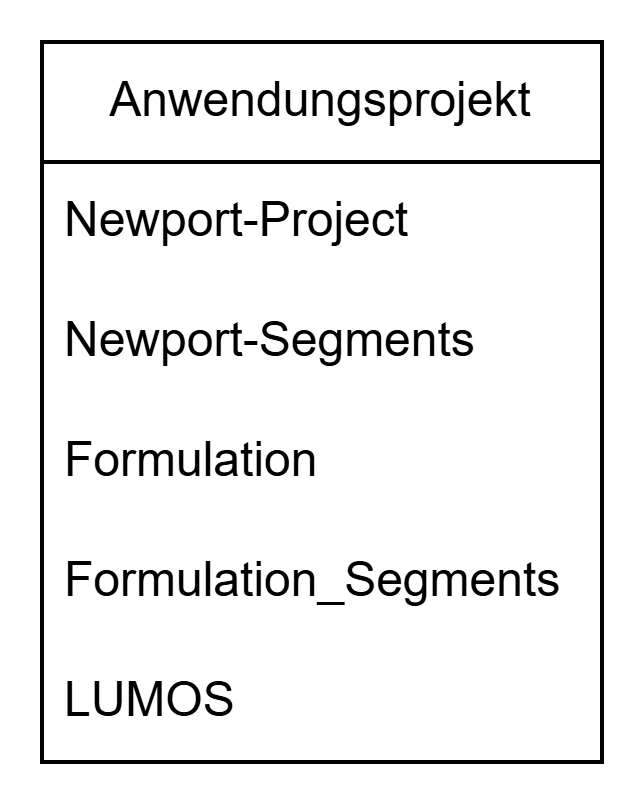
\includegraphics[width=\linewidth]{./img/projektGrafik.png}
\end{center}